\documentclass{article}
\usepackage{amsmath}
\usepackage{amssymb}
\usepackage{enumitem}
\usepackage{tikz}
\usepackage{forest}
\usepackage{graphicx}


\title{HW \#4}
\author{
    Uziel Rivera-Lopez
}
\date{03/26/2023}
\begin{document}
\maketitle
\section*{Problem 1}
\begin{enumerate}[label=(\alph*)]
    \item 
    \begin{enumerate}[label=\arabic*.]
        \item A = (1,1)
        \item B = (2,2)
        \item C = (2,4)
        \item D = (1,2)
    \end{enumerate}
    This table shows the euclidean distance between the points, using the formula $ d= \sqrt{(x_2 - x_1)^2 + (y_2 - y_1)^2}$.
    \begin{center}
        \begin{tabular}{|c|c|c|c|c|}
            \hline
            & A & B & C & D \\
            \hline
            A & 0 & 1.4142 & 3.1623 & 1 \\
            \hline
            B & 1.4142 & 0 & 2 & 1 \\
            \hline
            C & 3.1623 & 2 & 0 & 2.2361 \\
            \hline
            D & 1 & 1 & 2.2361 & 0 \\
            \hline
        \end{tabular}
    \end{center}
    \begin{enumerate}
        \item $Distance_{AB} = \sqrt{(2-1)^2 + (2-1)^2} = \sqrt{2} = 1.4142$
        \\$Distance_{AC} = \sqrt{(2-1)^2 + (4-1)^2} = \sqrt{10} = 3.1623$
        \\$Distance_{AD} = \sqrt{(1-1)^2 + (2-1)^2} = \sqrt{1} = 1$
        \item $Distance_{BA} = 1.4142$
        \\$Distance_{BC} = \sqrt{(2-2)^2 + (4-2)^2} = \sqrt{4} = 2$
        \\$Distance_{BD} = \sqrt{(1-2)^2 + (2-2)^2} = \sqrt{1} = 1$
        \item $Distance_{CA} = 3.1623$
        \\ $Distance_{CB} = 2$
        \\ $Distance_{CD} = \sqrt{(1-2)^2 + (2-4)^2} = \sqrt{5} = 2.2361$
        \item $Distance_{DA} = 1$
        \\$Distance_{DB} = 1$
        \\$Distance_{DC} = 2.2361$
    \end{enumerate}
    Now we can take min distance between the points and group them together to form the clusters. 
    \begin{enumerate}
        \item $min(AB, AC, AD) = AD$
        \item $min(BA, BC, BD) = BD$
        \item $min(CA, CB, CD) = CB$
        \item $min(DA, DB, DC) = DA or DB$
    \end{enumerate}
    \begin{tikzpicture}
        \draw[->] (0,0) -- (5,0);
        \draw[->] (0,0) -- (0,5); 
    
        \fill (1,1) circle (2pt) node[below right] {A};
        \fill (2,2) circle (2pt) node[below right] {B};
        \fill (2,4) circle (2pt) node[above] {C};
        \fill (1,2) circle (2pt) node[below right] {D};


        \draw (1,1) -- (2,2);
        \draw (1,1) -- (1,2);
        \draw (2,2) -- (2,4);
    \end{tikzpicture}
    \\Because CB is the only group cluster we do not consider it, as we see D, B and A are close to each other, giving us a better grouping of the data.
    So the clusters are:
    \begin{enumerate}
        \item A, D, B
        \item C
    \end{enumerate}
    \item \begin{figure}[h]
        \centering
        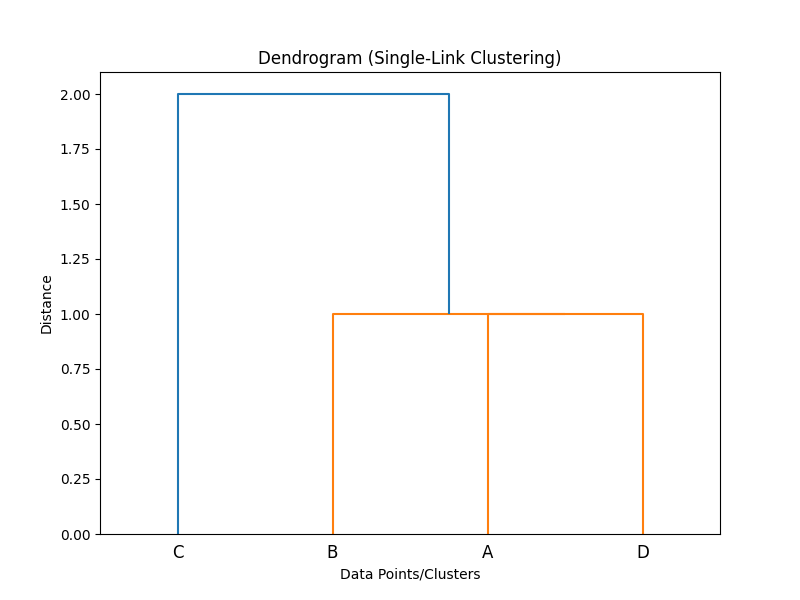
\includegraphics[width=0.5\textwidth]{Dendrogram.png}
    \end{figure}
\end{enumerate}
\section*{Problem 2}
\begin{enumerate}[label=(\alph*)]
    \item We want to tune our clustering based on the applications we are using it for, based off the book. This way we can
    have a better understanding of the data, and how our model is doing. Furthermore, we will have better use of the computing power and time, instead of
    taking more time on evalutating if we have the right number of clusters.
    
    \item Because if we have a lot of clusters, so take for example the problem 1, we have 4 points and we give
    each one their own cluster, then we would be underfitting the data. On the other hand, if we have too few clusters
    then we would be overfitting the data, in either case we can have a loss of information. Since we would have a loss of information or hard to read results, our interpretation of the data 
    would be affected as well, and we would also have a hard time making decisions based on the data. Also we would be wasting computing power and time.
\end{enumerate}
\section*{Problem 3}
\begin{enumerate}[label=(\alph*)]
    \item First off we need to calculate the distances from 4 to the other points
    \begin{enumerate}
        \item $ |4-2| = 2$
        \item $ |4-3| = 1$
        \item $ |4-5| = 1$
        \item $|4-7| = 3$
        \item $ |4-9| = 5$
        \item $[2,1,1,3,5]$
    \end{enumerate}
    Now the closest points are 3 and 5, so we can group them together. With the KNN density estimator we get:
    \\density = $\frac{k}{V_{k}(x)N} = \frac{2}{5\cdot V_{2}(x)}=?$
    \\Now this is the part I'm confused on but I think the $V_{k}(x) = 2$ Because since we are in a 1 dimensional space, the volume is the distance between the two points, so 2*r= 2*1 = 2.
    \\So the density is $\frac{2}{5\cdot 2} = 0.2$
    \item The same concept is applied here
    \begin{enumerate}
        \item $ |5-2| = 3$
        \item $ |5-3| = 2$
        \item $ |5-5| = 0$
        \item $|5-7| = 2$
        \item $ |5-9| = 4$
        \item $[3,2,0,2,4]$
    \end{enumerate}
    Since the k is now 3, we need 3 neighbors, so the closest are 5, 3, 7.
    \\density = $\frac{3}{5\cdot V_{3}(x)} = ?$
    Assuming what I said was correct then $V_{3}(x) = 2*2 = 4$
    \\So the density is $\frac{3}{5\cdot 4} = 0.15$
\end{enumerate}
\section*{Problem 4}
\begin{enumerate}[label=(\alph*)]
    \item Outliers are "anomalies" that are difference from what we expect. So something like in 
    Question 3b where we did x=5 and we already have 5 in the data set, so it would be a sort of anomaly
    \item Because outliers can affect the way we learn, it can also affect the way our models can learn. By implementing an outlier detection 
    we can make the density estimation for a dataset, while detecting the outliers that are very less probable. 
    \item LOF works by seeing the density from a point x to kth neighbors, $d_{k}(x)$ and then we use the 1 over the instances of in the x neighbors, $|N{x}|$ and multiply that by the average distances of some s in the $N{x}$, $d_{k}(s)$.
    The main idea with LOF is that we are comparing the densities of the neighbors to the average density of the neighbors.
\end{enumerate}
\section*{Problem 5}
\begin{enumerate}[label=(\alph*)]
    \item We need to divide the training data into bins of some size. Then using the origin of the dataset we can create intervals of the bins.
    Then we can use the amount in bins instead of the actual data. Then form the histogram of the data. Creating a histogram is a much more simply way of visualizing the data, and we can even determine how the h, size of division, affects 
    the histogram. They are also flexible since it doesn't assume any distribution of the data. Yet, since we can see the affects of the h, it also affects our density estimation. We are also sensitivtiy to where we start from, which is way we implemment naive estimator.
    Also we have a sort of limit as to how many dimensions we can go with the histogram. 
    \item The Kernel estimator is a method used to get a smooth estimate of the density of the data, it's also a nonparametric method like KNN. It sums the bumps of what was created by the function, just like how the naive estimate is the sum of the boxes. 
    It uses the points of $x^t$ to influence the estimate, and also determines the window width with the sizes of the bin, h, it also large effects on smaller region but no effects with distance x points. As stated, Kernel estimator is influenced by all the x points, while KNN we only care about the kth neighbors. The Kernel estimator is also more smooth than the KNN estimator. The Kernel aslo creats a much more smoother estimate of the density, while the KNN is more jagged. 
\end{enumerate}
\section*{Problem 6}
\begin{enumerate}[label=(\alph*)]
    \item We take the min value (1.2) and max value (6.1) to create the different bins.
    \begin{enumerate}
        \item $1.2 + 0.5 = 1.7$
        \item $1.7 + 0.5 = 2.2$
        \item $2.2 + 0.5 = 2.7$
        \item $2.7 + 0.5 = 3.2$
        \item $3.2 + 0.5 = 3.7$
        \item $3.7 + 0.5 = 4.2$
        \item $4.2 + 0.5 = 4.7$
        \item $4.7 + 0.5 = 5.2$
        \item $5.2 + 0.5 = 5.7$
        \item $5.7 + 0.5 = 6.2$
        \item Our bins: [1.2, 1.7), [1.7, 2.2), [2.2, 2.7), [2.7, 3.2), [3.2, 3.7), [3.7, 4.2), [4.2, 4.7), [4.7, 5.2), [5.2, 5.7), [5.7, 6.2]
    \end{enumerate}
    Then we determine the amount of points in each bin:
         [1.2, 1.7) = 1
         [1.7, 2.2) = 0
         [2.2, 2.7) = 2
         [2.7, 3.2) = 1
         [3.2, 3.7) = 1
         [3.7, 4.2) = 0
         [4.2, 4.7) = 1
         [4.7, 5.2) = 1
         [5.2, 5.7) = 2
         [5.7, 6.2) = 1
    \\Since our value will x=3 will be going in the bin [2.7, 3.2), we can calculate the density of the bin by dividing the amount of points in the bin by the total amount of points and the size, h, so $\frac{2}{10\cdot5} = 0.4$
    \item We need to determine how our data is distributed in terms of shape. If we have a circular shape, then we know a Gaussian kernel would be best. Yet, if it's an epliptical shape, then the ellipsoidal kernel would be a better choice to go with.
    Also the calculations of the Gaussian kernel is much more simpler, but the ellipsoidal kernel is more complex beause of the separate variance parameter in each dimension. However, the ellipsoidal gives us more flexibility because it allows for different variances, so it can capture much more complex shapes. While the Gaussian remains more constant throughout, and only capturing linear patterns.
    \item We first start off with an empty set, Z, then iteratre through the x points in the X dataset, determine the smallest distance between the x point and another point, then we add the x point to the z point. We then calculate the distance between the x point and the z point.
    Then repeat the process until we can't find a change in the Z subdataset.
\end{enumerate}
\end{document}